\section{Language and notation}
\subsection{Lexical elements}
\subsubsection{Character sets}

The Dats v2.0.0 language supports the 26 \textit{uppercase letters} and 26
\textit{lower case letter} of the \textit{Latin alphabet}:

\begin{verbatim}
       A B C D E F G H I J K L M
       N O P Q R S T U V W X Y Z
       a b c d e f g h i j k l m
       n o p q r s t u v w x y z
\end{verbatim}

the 10 {decimal digits}:
\begin{verbatim}
       0 1 2 3 4 5 6 7 8 9
\end{verbatim}

and the miscs symbols:
\begin{verbatim}
       - + * / ( ) { } [ ] " ; = . , #
\end{verbatim}

\subsubsection{Keywords}

\np Keywords: one of

\begin{verbatim}
       attack        bpm          track
       decay         filter       n
       main          mix          r
       octave        read
       release       semitone
       sustain       synth
       volume        write
\end{verbatim}

\subsubsection{Reserved words}

\np Reserved words: The Dats language prohibits the use of the
following words as an identifier:

\np The 70 unaccidented notes:

\begin{verbatim}
       a0 a1 a2 a3 a4 a5 a6 a7 a8 a9
       b0 b1 b2 b3 b4 b5 b6 b7 b8 b9
       c0 c1 c2 c3 c4 c5 c6 c7 c8 c9
       d0 d1 d2 d3 d4 d5 d6 d7 d8 d9
       e0 e1 e2 e3 e4 e5 e6 e7 e8 e9
       f0 f1 f2 f3 f4 f5 f6 f7 f8 f9
       g0 g1 g2 g3 g4 g5 g6 g7 g8 g9
\end{verbatim}

the 70 accidented \textit{flat notes} ($\flat$):

\begin{verbatim}
       ab0 ab1 ab2 ab3 ab4 ab5 ab6 ab7 ab8 ab9
       bb0 bb1 bb2 bb3 bb4 bb5 bb6 bb7 bb8 bb9
       cb0 cb1 cb2 cb3 cb4 cb5 cb6 cb7 cb8 cb9
       db0 db1 db2 db3 db4 db5 db6 db7 db8 db9
       eb0 eb1 eb2 eb3 eb4 eb5 eb6 eb7 eb8 eb9
       fb0 fb1 fb2 fb3 fb4 fb5 fb6 fb7 fb8 fb9
       gb0 gb1 gb2 gb3 gb4 gb5 gb6 gb7 gb8 gb9
\end{verbatim}

and the 70 accidented \textit{sharp notes}\footnote{By nature of the syntax of
the language, the use of \protect\texttt{\#} in an identifer is prohibited,
but it is mentioned here to be explicit.} ($\sharp$):
\begin{verbatim}
       a#0 a#1 a#2 a#3 a#4 a#5 a#6 a#7 a#8 a#9
       b#0 b#1 b#2 b#3 b#4 b#5 b#6 b#7 b#8 b#9
       c#0 c#1 c#2 c#3 c#4 c#5 c#6 c#7 c#8 c#9
       d#0 d#1 d#2 d#3 d#4 d#5 d#6 d#7 d#8 d#9
       e#0 e#1 e#2 e#3 e#4 e#5 e#6 e#7 e#8 e#9
       f#0 f#1 f#2 f#3 f#4 f#5 f#6 f#7 f#8 f#9
       g#0 g#1 g#2 g#3 g#4 g#5 g#6 g#7 g#8 g#9
\end{verbatim}

a total of 210 reserved words.


\subsubsection{Future reserved words}

\np Future reserved words: composers must execise caution from using any
of the following words:

the 70 accidented \textit{double flat notes} ($\flat\flat$):

\begin{verbatim}
       abb0 abb1 abb2 abb3 abb4 abb5 abb6 abb7 abb8 abb9
       bbb0 bbb1 bbb2 bbb3 bbb4 bbb5 bbb6 bbb7 bbb8 bbb9
       cbb0 cbb1 cbb2 cbb3 cbb4 cbb5 cbb6 cbb7 cbb8 cbb9
       dbb0 dbb1 dbb2 dbb3 dbb4 dbb5 dbb6 dbb7 dbb8 dbb9
       ebb0 ebb1 ebb2 ebb3 ebb4 ebb5 ebb6 ebb7 ebb8 ebb9
       fbb0 fbb1 fbb2 fbb3 fbb4 fbb5 fbb6 fbb7 fbb8 fbb9
       gbb0 gbb1 gbb2 gbb3 gbb4 gbb5 gbb6 gbb7 gbb8 gbb9
\end{verbatim}

the 70 accidented \textit{double sharp notes} ($\sharp\sharp$):

\begin{verbatim}
       a##0 a##1 a##2 a##3 a##4 a##5 a##6 a##7 a##8 a##9
       b##0 b##1 b##2 b##3 b##4 b##5 b##6 b##7 b##8 b##9
       c##0 c##1 c##2 c##3 c##4 c##5 c##6 c##7 c##8 c##9
       d##0 d##1 d##2 d##3 d##4 d##5 d##6 d##7 d##8 d##9
       e##0 e##1 e##2 e##3 e##4 e##5 e##6 e##7 e##8 e##9
       f##0 f##1 f##2 f##3 f##4 f##5 f##6 f##7 f##8 f##9
       g##0 g##1 g##2 g##3 g##4 g##5 g##6 g##7 g##8 g##9
\end{verbatim}

\subsubsection{Identifier}


\subsubsection{Intrinsic functions}

\subsubsection{Note}

\np \textbf{Syntax}

\begin{verbatim}
<note> : [a-g](#|b)?[0-9] <symbols>
       | <note> "," <note>
<symbols> : <staccatto>
          | <staccatissmo>
          |
          ;
<staccatto> : "."
            ;
<staccatissimo> : "_"
                ;
\end{verbatim}

\subsubsection{Length}

\subsubsection{Comments}
\np Just like in the C programming language, you can use a double slash (solidus if you like), \verb+//+.
It eats the letters/words in its front until it reaches a newline.
\begin{Verbatim}[frame=single]
      staff foo {
        n 1, c4; //EAT MEEE!!!
      }
\end{Verbatim}

\subsection{Declarations}

\subsection{\texttt{staff}}
\np The \textgray{staff} keyword signifies the beginning of a staff. It is then followed by an identifier and \verb+{+. A staff consist of
musical notes and musical rests which is declared by using \verb+n+, or \verb+r+, inside the \textit{staff block}.
The staff, is terminated by \verb+}+. The, \verb+n+, or, \verb+r+, which is declared inside the \textit{staff block} both takes an argument.

\subsubsection{\texttt{n}}

\np The \verb+n+ keyword signifies the beginning of a musical note. It must be declared
inside the staff block.
It takes 2 parameters; the \textgray{<length>} and the \textgray{<note>} of the
musical note, each separated by a comma. It must end with a semicolon: 

\begin{Verbatim}[frame=single]
      n <length>, <note>;
\end{Verbatim}

\paragraph{\texttt{<note>}} The parameter \textgray{<note>} consist of a \verb+key+ and an \verb+octave+. It shall be in the form of \verb+[a-g](#|b)?[0-9]+:

\begin{Verbatim}[frame=single]
  c4 // [abcdefg](b|#)?[0-9]
  ||
  |`--->octave 4
  v
 key 'c'
\end{Verbatim}
The above has a key 'c' at octave 4.

\np To play a whole note ringing at c4:
\begin{Verbatim}[frame=single]
      staff foo {
        n 1, c4;
      }
\end{Verbatim}

\begin{center}
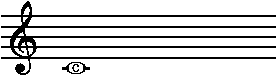
\includegraphics{notes/1c}
\end{center}

a half of a note ringing at d4:

\begin{Verbatim}[frame=single]
      staff foo {
        n 2, d4;
      }
\end{Verbatim}

\begin{center}
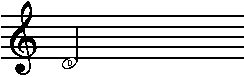
\includegraphics{notes/2d}
\end{center}

and a quarter of a note ringing at e4:
\begin{Verbatim}[frame=single]
      staff foo {
        n 4, e4;
      }
\end{Verbatim}

\begin{center}
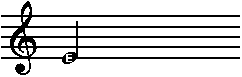
\includegraphics{notes/4e}
\end{center}

\np One can derive the length of the note from the denominator of these notes:
\verb+1/1 1/2 1/4+

\subparagraph{dyad}
The parameter \textgray{<note>} may be entered for a number of times:

\begin{Verbatim}[frame=single]
      staff foo {
        n 4, c4 e4 g4;
      }
\end{Verbatim}

\begin{center}
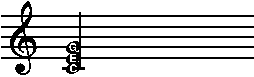
\includegraphics{notes/dyad_ceg}
\end{center}

\np The example above plays the C major chord at root position as whole note. (Integer overflow is not
protected; you might hear undesirable sounds.)

\np Dotted notes are implemented which reduces the duration of the playing of
that note. To use dots, you must to use a period. An example below is a 1/4 dotted note:
\begin{Verbatim}[frame=single]
      staff foo {
        n 4., c4;
        n 4..,d4;
      }
\end{Verbatim}

\begin{center}
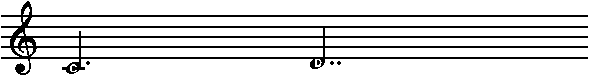
\includegraphics{notes/cpdpp}
\end{center}

\np There is no limit on how many dots you can enter; what's stopping you
is the limit to what the human ears can recognized.

\np The key from A-G is supported, and the octave it takes must be an integer
from 0 to 9.

\np To use accidentals, append \verb+#+ to the first letter of the note to raise the note a semitone and to lower the
note a semitone, append \verb+b+ to the first letter of the note:
\begin{Verbatim}[frame=single]
      staff foo {
        n 1, c#4;
        n 2, db4;
      }
\end{Verbatim}

\begin{center}
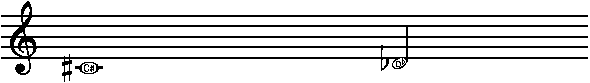
\includegraphics{notes/csdf}
\end{center}

\np Unlike the parameter \textgray{length>}, arithmetic operation is illegal
to perform on a \textgray{<note>}. so \textgray{<note>+<note>} is prohibited.

\np To play a chord or a dyad, like \textgray{c4 e4 g4}, one just needs to write as it is:

\begin{Verbatim}[frame=single]
      n 4, c4 e4 g4;
\end{Verbatim}

\textbf{NOTE} If all these notes is played as staccato, append,
\textgray{.}, to them, so, it becomes, \textgray{c4. e4. g4.}

\paragraph{\texttt{<length>}} For argument, \textgray{<length>}, it may be in the form of integer or floating point number:
\label{nlength}

\begin{Verbatim}[frame=single]
      n 4.0, <note>;
      n 4, <note>;
\end{Verbatim}

\np To simulate a tie, use \verb-+-

\begin{Verbatim}[frame=single]
      n 4+4, 440; /* is equivalent to: */
      n 2, 440; 
\end{Verbatim}

\np How the former is equivalent to \textgray{n 2, 440;} might
not make sense as, $4+4$ is mathematically equal to 8. Instead
of treating this as an addition operation which sums up two
operands (which is confusing), consider to pronouce it as
\textit{four-tie-four} instead of \textit{four-plus-four}.
 
\textbf{NOTE} Other arithmetic operations are prohibited.

\np The paramater, \textgray{<length>}, will take any real positive integer (as long as it's in the range of int),
so a length of \verb+3+ will work (equivalent to 1/3 of a note), \verb+5+ will work (equivalent to 1/5
of a note) and others.

\np To play a 1/8 note triplet, one may need to do some math:

\begin{align}
	\shortintertext{Multiply 1/8 with 2:}
	\frac{1}{8}2 = \frac{2}{8} \Rightarrow \frac{1}{4} \\
	\shortintertext{divide the answer with 3 (3 for triplet):}
	\frac{1}{4(3)} = \frac{1}{12}
\end{align}

and use the denominator, \verb+12+, as the value of the length:
\begin{Verbatim}[frame=single]
      staff foo {
        n 12, c4;
        n 12, d4;
        n 12, e4;
      }
\end{Verbatim}

\begin{center}
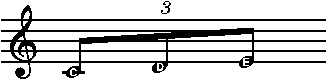
\includegraphics{notes/4triplet_cde}
\end{center}

This process can be repeates for 1/8 note quadruplet, but instead of dividing
with 3 in step (2), it's divided with 4 (4 for quadruplet) and so on.


\subsubsection{\texttt{r}}

\np The \verb+r+ keyword signifies the beginning of a musical rest. It must be
declared inside the \textit{staff block}. It takes one parameter; the
length of the rest:

\begin{Verbatim}[frame=single]
      r <length>;
\end{Verbatim}

\np The syntax of \textgray{<length>} is similar to the definition in 
\autoref{nlength}.

\subsubsection{Extensions}

\subsection{\texttt{track}}
\np A declaration of variable of type,
\verb+track+, must be immdediately followed by its identifier, followed by
an assignment to one of synthesizers taking a type, \verb+staff+. 
\begin{Verbatim}[frame=single]
       track foo = synth.psg(pol);
\end{Verbatim}

or other variable of type ,\verb+track+.
\begin{Verbatim}[frame=single]
      track foo = synth.psg(pol);
      track bar = foo;
\end{Verbatim}

\np To append these supported types, a comma must be added, followed by an rvalue:
\begin{Verbatim}[frame=single]
      track foo = synth.psg(bar), synth.psg(bar);
\end{Verbatim}


\subsubsection{Extensions}

\np The length of the rest is semantically similar to one of that length
of the note. Refer to the \verb+n+ keyword.

\subsection{Formatting}
\label{formatting}
\np To preserve the readability of the text, it is a recommended practice to add a comment for every
beginning measure, regardless of the time signature. Below is a 4/4 time signature:
\begin{Verbatim}[frame=single]
      staff foo {
        // Measure 1
        n 1, c4;
  
        // Measure 2
        n 4, d4;
        n 4, e4;
        n 4, f4;
        n 4, g4;
  
        // Measure 3
        n 2, a4;
        n 2, b4;
      }
\end{Verbatim}

